\documentclass{beamer}
\usepackage{UCLAbeamer}
\usepackage{color}

%import citation package 
%\usepackage[maxnames=100]{biblatex}
\addbibresource{bibliography.bib}
\usepackage{transparent}
\usepackage{booktabs} 
\usepackage{tabularx}
\usepackage{makecell}

%%% To add citations
%\usepackage[
%backend=biber,
%style=alphabetic,
%]{biblatex}
\renewcommand*{\bibfont}{\normalfont\fontsize{5}{5}\selectfont}
%\usepackage{algorithm}
%\usepackage{algpseudocode}
%\usepackage{lipsum}
%\usepackage{hyperref}


%Information to be included in the title page:
\title{Unveiling the Parallel Function Hypothesis on Personal Pronouns: A Corpus Analysis Utilizing Eye-Tracking Data}
\author{Yue Chen}
\institute{University of California, Los Angeles}
\subtitle{The 11th Conference on Language, Discourse, and Cognition (CLDC11)}
\date{May 4th 2024}


\begin{document}

\frame{\titlepage}

\begin{frame}
\begin{figure}
    \centering

\includegraphics[width=5cm,keepaspectratio]{figures/qr-code.png}
\end{figure}
\end{frame}


\begin{frame}
\frametitle{Background}
\begin{itemize}
\item This study investigates the influence of the Parallel Functioning Hypothesis on first fixation duration, number of fixations, and number of skips during sentence processing by using the LARC-ID eye-tracking dataset \cite{harris2021angeles}
\end{itemize}
\end{frame}


\begin{frame}
\frametitle{Parallel Functioning Hypothesis (PFH)}
\begin{itemize}
    \item In complex sentences, the presence of the pronoun and its referential noun phrases (NPs) within the same grammatical functional category leads to Parallel Function Pronoun Resolution (PFR) \cite{sheldon1974role}\cite{grober1978parallel}
    \item PFR results in easier and quicker processing when the pronouns and their referents fall into the same grammatical function category (Parallel Function), compared to Non-Parallel Function Pronoun Resolution (NPFR) \cite{cinkara2015parallel}\cite{sheldon1974role}\cite{grober1978parallel}
    \item This phenomenon has been observed in both adults and children, indicating that participants of all ages benefit from the Parallel Functioning Hypothesis by experiencing reduced processing time for pronoun resolution \cite{arnold2015effects}\cite{chien1990children}
\end{itemize}
\end{frame}

\begin{frame}{Grammatical Function Type (Parallel and Nonparallel Function)}
    \begin{table}[]
        \centering\small
        \begin{tabular}{p{1.5cm}p{1.5cm}p{1cm}p{5.5cm}}
        \hline\hline
            Pronoun Grammatical Function & Antecedent NP Function & Sentence Label & Sentence Example \\\hline
            Subject & Subject & Parallel & \textbf{Nathan} disliked Aron and similarly, \textbf{he} hated Nicole for a while and in the end, they all avoided each other\\
            Subject&Object&Non-Parallel&
            \textbf{Fiona} defeated in the court and so James congratulated \textbf{her} after the match but nobody took any notice.
          \\\hline\hline
        \end{tabular}
        \caption{Examples of Parallel and Non-Parallel Sentences}
        \label{Table: Examples of Parallel and Non-Parallel Sentences}
    \end{table}
\end{frame}

\begin{frame}
\frametitle{Pronoun Interpretation}
\begin{itemize}
\item Pronoun interpretation is influenced by both linguistic contexts, such as syntactic structures, social cues, eye gaze, and physical gestures  \cite{arnold2015effects} \cite{chien1990children}
\item People employ previous linguistic experiences, context, linguistic cues, gender, number, pragmatics, and semantics to disambiguate pronoun understanding \cite{sorlin2015pragmatics}\cite{oshima1988children}
\item People experience significantly increasing processing time of an intar-sentential sentence compared to an inter-sentential sentence \cite{brennan1987centering}

\end{itemize}
\end{frame}

\begin{frame}{Sentence Type (Intrasentential and Intersentential)}
    \begin{table}[]
        \centering\small
        \begin{tabular}{p{1.5cm} p{7cm}}
        \hline\hline
           Sentence Label & Sentence Example \\\hline
            Intra & \textbf{Lemuel} knew most of their faces by now, and even some of their names. They didn't let on that they noticed \textbf{him}, and maybe they didn't see \textbf{him} at all.\\
            Inter&
            \textbf{Lemuel} sat down just out of her reach and tried to say \textbf{he} was sorry, but nothing would come.
          \\\hline\hline
        \end{tabular}
        \caption{Examples of Intra and Inter Sentences}
        \label{tab:Examples of Intra and Inter Sentences}
    \end{table}
\end{frame}

\begin{frame}{Sentence Type (SO, SS, OS)}
    \begin{table}[]
        \centering\small
        \begin{tabular}{p{1.5cm}p{1.5cm}p{1cm}p{5.5cm}}
        \hline\hline
            Antecedent NP Function & Pronoun Grammatical Function & Sentence Label &Sentence Example \\\hline
            Subject & Object & SO & \textbf{Lemuel} pondered the dots for some time, avoiding the extreme right-hand edge of the map, thinking that perhaps he would like to visit a place where everyone was very small. But in the photographs the people looking back at \textbf{him} seemed to be the same size as anyone else.\\
            Subject&Subject&SS&\textbf{Lemuel} knew that if he was with her she'd have to slow down for him\\
            Object&Subject&OS&If a thing like that touched him at all, Lemuel thought - but he could not imagine what would happen then.\\\hline\hline
        \end{tabular}
        \caption{Examples of SO, SS, OS Sentence}
        \label{tab:Examples of SO, SS, OS Sentences}
    \end{table}
\end{frame}

\begin{frame}
\frametitle{Research Question}
\begin{itemize}
    \item From a naturalistic reading perspective will the personal pronoun regulation obey the Parallel Functioning Hypothesis?
    \item Will the different grammatical functions of personal pronouns (SS, SO, OS) influence how people process referents?
    \item Will different sentence structures (inter and intar) influence how people process referents?
    \item How do previous knowledge and experiences influence an individual's pronoun resolution?

\end{itemize}
\end{frame}

\begin{frame}
\frametitle{Data Set}
\begin{itemize}
    \item This study utilized the LARC-ID eye-tracking dataset \cite{harris2021angeles} 
    \item 15 participants (10 females, 5 males) were recruited for the LARC-ID dataset
    \item All participants were native English speakers with a mean age of 19 years (SD = 1.13 years), ranging from 18 to 22 years
    \item All participants had some college experience, with an average of 2 years (range: 1-4 years)
\end{itemize}
\begin{figure}
    \centering
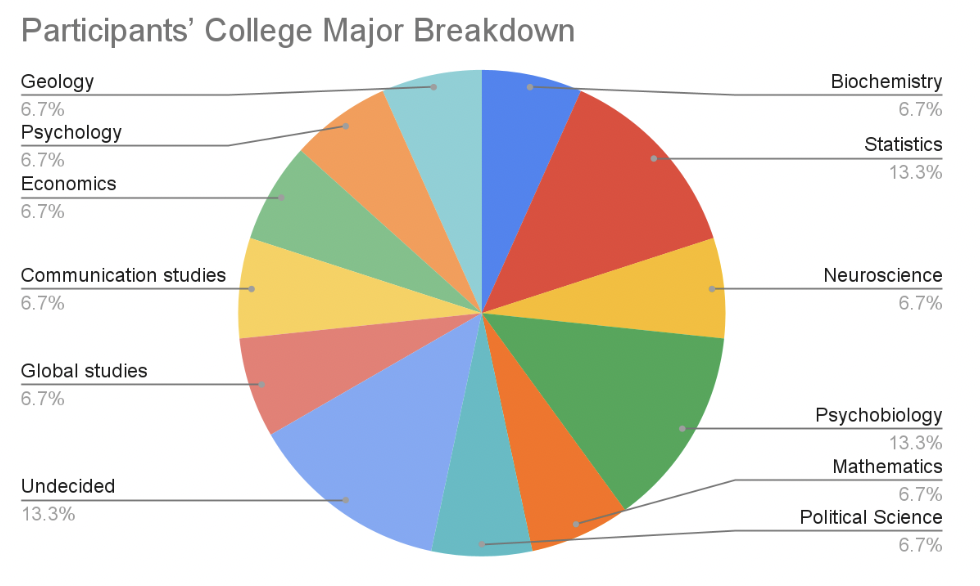
\includegraphics[width=6cm,keepaspectratio]{figures/demographics.png}
    \caption{Participants Demographics}
    \label{Figure:Participants Demographics}
\end{figure}
\end{frame}

\begin{frame}
\frametitle{Data Annotation}
\begin{itemize}
    \item In total, 12 sentences were selected
         \begin{itemize}
         \item 6 PF sentence and 6 NPF sentences
         \item 6 PF sentence and 6 NPF sentences
         \end{itemize}
    \item Four main areas of a sentence
     \begin{itemize}
        \item Target subject (the referent of the pronoun)
       \item  Target pronoun
       \item  Pronoun Region A (two words before the target pronoun)
       \item  Pronoun Region B (two words after the target pronoun)
      \end{itemize}
\end{itemize}
\textbf{Example From the Corpus}\\
If a thing like {\color{red}{\textbf{that touched}}} (Pronoun Region A) \textbf{him} (Target Pronoun) at all, \textbf{and sometimes} (Pronoun Region B) \textbf{Lemuel} (Target Subject) thought - but he could not imagine what would happen then.
\end{frame}


\begin{frame}
\frametitle{Result}
\begin{itemize}
    \item PF vs. NPF Sentences:
\begin{itemize}
    \item Slight differences in first fixation duration were observed between Parallel Function (PF) and Non-Parallel Function (NPF) sentences.
    \item More skips are seen in PF sentences compared to NPF sentences.
\end{itemize}
\end{itemize}
\begin{figure}
    \centering
    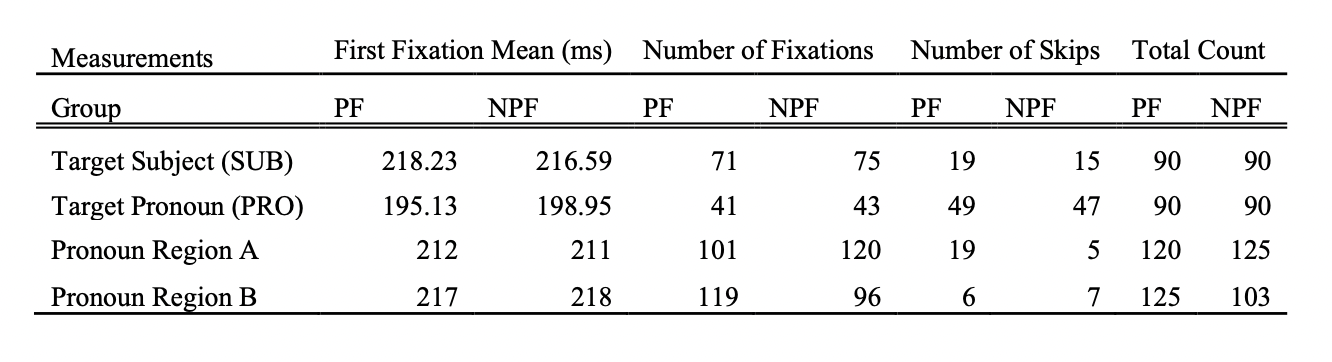
\includegraphics[width=9cm,keepaspectratio]{figures/first_fixation.png}
    \caption{PF and NPF Comparison}
    \label{table:PF and NPF Comparison}
\end{figure}
\end{frame}

\begin{frame}
\frametitle{Result}
\begin{itemize}
\item SS, SO, and OS Structures:
\begin{itemize}
 \item Subject-subject (SS) structures were most common, followed by subject-object (SO), and least common was object-subject (OS)
 \item In SO structures, the subject had the longest first fixation duration, while the target pronoun had the shortest
 \item Pronoun region B in SO structures had the longest first fixation duration
 
\end{itemize}
\end{itemize}
\begin{figure}
    \centering
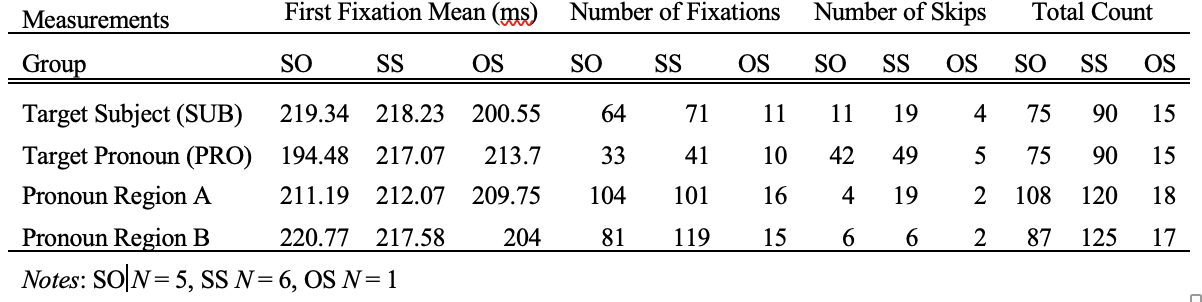
\includegraphics[width=9cm,keepaspectratio]{figures/SO_SS_OD.png}
    \caption{SO SS and OS Comparison}
    \label{table:SO SS and OS Comparison}
\end{figure}
\end{frame}

\begin{frame}
\frametitle{Result}
\begin{itemize}
 \item Intra vs. Inter-sentential Sentences:
 \begin{itemize}
 \item Intra-sentential structures had longer first fixation duration compared to inter-sentential structures.
 \item More skips occurred in inter-sentential structures.
\end{itemize}
\end{itemize}
 \begin{figure}
    \centering
    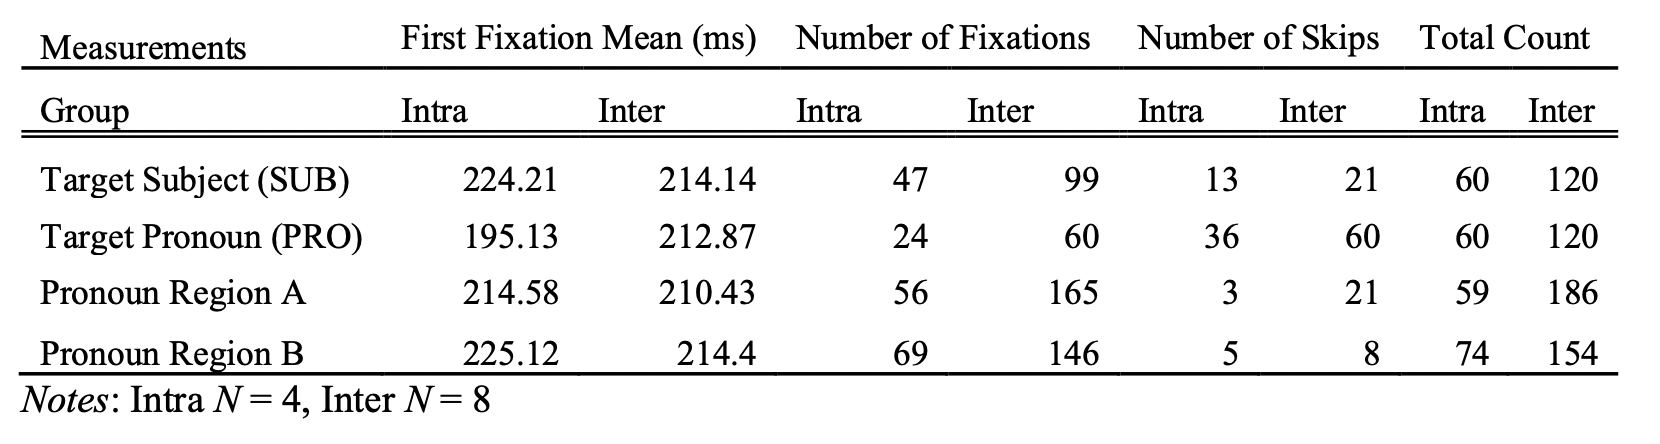
\includegraphics[width=9cm,keepaspectratio]{figures/Inter_Intra.png}
    \item \caption{Inter and Intra Sentence Comparison}
    \label{table:Inter and Intra Sentence Comparison}
\end{figure}
\end{frame}

\begin{frame}
\frametitle{Discussion}
\begin{itemize}
    \item The findings suggest that participants might use the grammatical positions of the target subject and pronouns as cognitive strategies for allocating processing resources based on the position of pronouns and their referents, which align with previous research on pronoun resolution, highlighting the role of salience and contextual cues in guiding participants' processing and interpretation \cite{arnold2015effects}\cite{brennan1987centering}\cite{garnham2013mental}
    \item The salience and position of the referent impact the processing dynamics of pronouns within a sentence \cite{macdonald2013language}
    \item The frequency of specific sentence structures in natural languages may also influence participants' processing time. More frequent structures are processed more efficiently due to participants' linguistic experience \cite{montag2015text}\cite{tanenhaus1995sentence}
\end{itemize}
\end{frame}

\section{Conclusion}
    \begin{frame}{Conclusion}
    \begin{itemize}
    \item There are minimal differences between Parallel Function and Non-Parallel Function sentences, failing to provide positive support in favor of this hypothesis. 
    \item The intrasentential structures lead to longer first fixation duration for the target subject, target pronoun, and both pronoun regions compared to intersentential structures. 
    \item The grammatical positions of the subjects and the pronouns indicate that when the subject and pronoun are in the subject-object position, participants exhibit longer first fixation duration at the subject and shorter first fixation duration at the target pronoun.
    \end{itemize}
    \end{frame}


\begin{frame}
\frametitle{References}
    \printbibliography
    \end{frame}


\begin{frame}
\frametitle{Acknowledgement}
I am deeply grateful to my undergraduate thesis supervisor Dr. Jesse Harris from UCLA for his guidance and help throughout this project; Dr. Stephanie Rich for her help with data collection; the UCLA linguistics department for providing financial support for this project; all members of the UCLA language processing lab for their comments and suggestions and the participants who participated in this study.
\end{frame}

\end{document}
